\documentclass[12pt,twoside]{article}
\usepackage[utf8x]{inputenc}

%%%%%%%%%%%%%%%%%%%%%%%%%%%%%%%%%%%%%%%%%%%%%%%%%%%%%%%%%%%%%%%%%%%%%%%%%%%%%

% Definitions for the title page
% Edit these to provide the correct information
% e.g. \newcommand{\reportauthor}{Timothy Kimber}

\newcommand{\reporttitle}{Theory and simulation of quantum information processing with trapped ions}
\newcommand{\reportauthor}{Lajos Palanki}
\newcommand{\supervisor}{Prof. Richard Thompson}
\newcommand{\degreetype}{MSc Physics}
\newcommand{\projectcode}{QOLS-Thompson-1}
\newcommand{\CID}{01496799}
\newcommand{\assessor}{Dr Steve Kolthammer}

%%%%%%%%%%%%%%%%%%%%%%%%%%%%%%%%%%%%%%%%%%%%%%%%%%%%%%%%%%%%%%%%%%%%%%%%%%%%%

% load some definitions and default packages
%%%%%%%%%%%%%%%%%%%%%%%%%%%%%%%%%%%%%%%%%
% University Assignment Title Page 
% LaTeX Template
% Version 1.0 (27/12/12)
%
% This template has been downloaded from:
% http://www.LaTeXTemplates.com
%
% Original author:
% WikiBooks (http://en.wikibooks.org/wiki/LaTeX/Title_Creation)
%
% License:
% CC BY-NC-SA 3.0 (http://creativecommons.org/licenses/by-nc-sa/3.0/)
% 
%
%%%%%%%%%%%%%%%%%%%%%%%%%%%%%%%%%%%%%%%%%
%----------------------------------------------------------------------------------------
%	PACKAGES AND OTHER DOCUMENT CONFIGURATIONS
%----------------------------------------------------------------------------------------
\usepackage[a4paper,hmargin=2.5cm,vmargin=2cm,includeheadfoot]{geometry}
\usepackage{textpos}
\usepackage{cite} % for bibliography
\usepackage{tabularx,longtable,multirow,subcaption,caption,wrapfig}%hangcaption
\usepackage{fncylab} %formatting of labels
\usepackage{fancyhdr} % page layout
\usepackage{url} % URLs
\usepackage[english]{babel}
\usepackage{amsmath}
\usepackage{amsfonts}
\usepackage{graphicx}
\usepackage{dsfont}
\usepackage{epstopdf} % automatically replace .eps with .pdf in graphics
\usepackage{backref} % needed for citations
\usepackage{array}
\usepackage{latexsym}
\usepackage[pdftex,pagebackref,hypertexnames=false,colorlinks]{hyperref} % provide links in pdf

\hypersetup{pdftitle={},
  pdfsubject={}, 
  pdfauthor={},
  pdfkeywords={}, 
  pdfstartview=FitH,
  pdfpagemode={UseOutlines},% None, FullScreen, UseOutlines
  bookmarksnumbered=true, bookmarksopen=true, colorlinks,
    citecolor=black,%
    filecolor=black,%
    linkcolor=black,%
    urlcolor=black}

\usepackage[all]{hypcap}


%\usepackage{color}
%\usepackage[tight,ugly]{units}
%\usepackage{float}
%\usepackage{tcolorbox}
%\usepackage[colorinlistoftodos]{todonotes}
% \usepackage{ntheorem}
% \theoremstyle{break}
% \newtheorem{lemma}{Lemma}
% \newtheorem{theorem}{Theorem}
% \newtheorem{remark}{Remark}
% \newtheorem{definition}{Definition}
% \newtheorem{proof}{Proof}


%%% Default fonts
\renewcommand*{\rmdefault}{bch}
\renewcommand*{\ttdefault}{cmtt}



%%% Default settings (page layout)
\setlength{\parindent}{0em}  % indentation of paragraph

\setlength{\headheight}{14.5pt}
\pagestyle{fancy}
\renewcommand{\chaptermark}[1]{\markboth{\chaptername\ \thechapter.\ #1}{}} 

\fancyfoot[ER,OL]{\sffamily\textbf{\thepage}}%Page no. in the left on odd pages and on right on even pages
\fancyfoot[OC,EC]{\sffamily }
\renewcommand{\headrulewidth}{0.1pt}
\renewcommand{\footrulewidth}{0.1pt}
\captionsetup{margin=10pt,font=small,labelfont=bf}


%--- chapter heading

\def\@makechapterhead#1{%
  \vspace*{10\p@}%
  {\parindent \z@ \raggedright \sffamily
    \interlinepenalty\@M
    \Huge\bfseries \thechapter \space\space #1\par\nobreak
    \vskip 30\p@
  }}

%---chapter heading for \chapter*  
\def\@makeschapterhead#1{%
  \vspace*{10\p@}%
  {\parindent \z@ \raggedright
    \sffamily
    \interlinepenalty\@M
    \Huge \bfseries  #1\par\nobreak
    \vskip 30\p@
  }}

\allowdisplaybreaks

\newcommand{\der}[3][]{\frac{\text{d}^{#1}#2}{\text{d}#3^{#1}}}
\newcommand{\partder}[3][]{\frac{\partial^{#1}#2}{\partial#3^{#1}}}
\newcommand{\expon}[2]{#1\cdot 10^{#2}}
\newcommand{\figref}[1]{Figure \ref{#1}}
\newcommand{\eref}[1]{Equation \eqref{#1}}
\newcommand{\tabref}[1]{Table \ref{#1}}
\newcommand{\result}[3]{$#1 \pm #2\,\text{#3}$}
\newcommand{\resexp}[4]{$\expon{(#1 \pm #2)}{#4}\,\text{#3}$}
\newcommand{\absresult}[3]{$\mathbf{#1 \pm #2\,\text{#3}}$}
\newcommand{\absresexp}[4]{$\mathbf{\expon{(#1 \pm #2)}{#4}\,\text{#3}}$}

\usepackage[export]{adjustbox}
\usepackage{pdfpages}
\usepackage{pgf}
\usepackage{relsize}
\usepackage{hyperref}

\graphicspath{{Images/}}

% load some macros
%\input{notation}

\date{Oct 2021}

\begin{document}

% load title page
% Last modification: 2015-08-17 (Marc Deisenroth)
\begin{titlepage}

\newcommand{\HRule}{\rule{\linewidth}{0.5mm}} % Defines a new command for the horizontal lines, change thickness here


%----------------------------------------------------------------------------------------
%	LOGO SECTION
%----------------------------------------------------------------------------------------

\includegraphics[width = 6cm]{./imperial}\\[0.5cm] 

\center % Center remainder of the page

%----------------------------------------------------------------------------------------
%	HEADING SECTIONS
%----------------------------------------------------------------------------------------

\textsc{\Large Imperial College London}\\[0.5cm] 
\textsc{\large Department of Physics}\\[0.5cm] 

%----------------------------------------------------------------------------------------
%	TITLE SECTION
%----------------------------------------------------------------------------------------

\HRule \\[0.4cm]
{ \huge \bfseries \reporttitle}\\ % Title of your document
\HRule \\[1.5cm]
 
%----------------------------------------------------------------------------------------
%	AUTHOR SECTION
%----------------------------------------------------------------------------------------

\begin{minipage}{0.4\textwidth}
\begin{flushleft} \large
\emph{Author CID:}\\
\CID\\
\vspace*{1em}
\emph{Project code:}\\
\projectcode
\end{flushleft}
\end{minipage}
~
\begin{minipage}{0.4\textwidth}
\begin{flushright} \large
\emph{Supervisor:} \\
\supervisor\\ % Supervisor's Name
\vspace*{1em}
\emph{Assessor:}\\
\assessor
\end{flushright}
\end{minipage}\\[4cm]

\vspace*{2em}
\begin{center}
	\emph{Word Count:}\\
	8019
\end{center}

%----------------------------------------------------------------------------------------
%	FOOTER & DATE SECTION
%----------------------------------------------------------------------------------------
\vfill % Fill the rest of the page with whitespace
Submitted as part of 
\degreetype~degree of Imperial College London\\[0.5cm]

\makeatletter
\@date 
\makeatother


\end{titlepage}




% page numbering etc.
\pagenumbering{roman}
\clearpage{\pagestyle{empty}\cleardoublepage}
\setcounter{page}{1}
\pagestyle{fancy}

\vspace*{\fill}
\begin{abstract}
In the present work I discuss the basic framework behind the operation of ideal Penning and Paul traps.  I then move on to discuss the theory behind laser cooling such trapped ions, via resolved sideband cooling. Finally a general overview of how such an ion trap can be used to simulate quantum gates is given, as well as highlighting some of the advancement that has occurred in the last decade in this field. These are essential in understanding how such a system might be simulated, and its imperfections taken into account.
\end{abstract}
\vspace*{\fill}
\newpage
%%%%%%%%%%%%%%%%%%%%%%%%%%%%%%%%%%%%

%%%%%%%%%%%%%%%%%%%%%%%%%%%%%%%%%%%%
%\section*{Acknowledgments}

%Comment this out if not needed.
%\clearpage{\pagestyle{empty}}

%%%%%%%%%%%%%%%%%%%%%%%%%%%%%%%%%%%%
%--- table of contents
\fancyhead[RE,LO]{\sffamily {Table of Contents}}
\tableofcontents
%\newpage
%\listoffigures
%\listoftables 

\clearpage{\pagestyle{empty}\cleardoublepage}
\pagenumbering{arabic}
\setcounter{page}{1}
\fancyhead[LE,RO]{\slshape \rightmark}
\fancyhead[LO,RE]{\slshape \leftmark}

%%%%%%%%%%%%%%%%%%%%%%%%%%%%%%%%%%%%
\section{Introduction}
\label{Intro}

Atoms and their interaction with light have been extensively studied in the past\cite{Foot,Woodgate}. Ion traps allow us to exploit this well studied interaction, and experiment with exotic states of matter\cite{Thompson_Coulomb_Crystals,Dipole_trap_BEC}; as well as use it to model quantum gates, further making advances into the field of quantum information processing\cite{Cold_trapped_ions_QC}.

In this present work I focus on exploring the various aspects required to perform and simulate quantum gate operations on trapped ions, such as the operation of the traps as well as the cooling required for such operations. Finally an overview of quantum information processing is presented.

This is to prepare work on simulating non-ideal systems within a framework like \cite{QuTip1,QuTip2}; in an effort to further understand the problems arising in experiments involving entangled trapped ions. Such models would allow mitigations against problems that limit the fidelity or even the feasibility of such experiments.

\section{Trapping techniques}
\label{Trap}

\subsection{Penning trap}
\label{Trap:Penning}

The first trap, which is of interest to us is the Penning Trap. In this device a combination of electrostatic and magnetostatic fields. A simple diagram of such a trap can be seen in \figref{Fig:Penning}. The ideal trap has a geometric structure, which follows $2z^2 -x^2 -y^2 = -r_0^2$ for the ring electrode and $2z^2 -x^2 -y^2 = 2z_0^2$ for the endcaps\cite{Charged_Particle_traps_Penning}. With a voltage differential of $V_0$ applied between the endcaps and the ring electrode, the electric potential will have the form\cite{Charged_Particle_traps_Penning,Penning_traps}:


\begin{figure}[!b]
	\centering
	\includegraphics[width=0.5\linewidth]{Penning_trap}
	\caption[Diagram of a Penning trap]{Cross section of a Penning trap. A magetic field, paralell to the axis of the trap leads to confinement in the plane normal to the axis; an electrostatic field generated by the electrodes confines the particle in the direction of the axis. This figure was taken from \cite{Penning_traps}}
	\label{Fig:Penning}
\end{figure}


\begin{equation}
	\Phi = \frac{V_0}{2d}\left(2z^2-x^2-y^2\right)
\label{Eq:Penning_EPot}
\end{equation}

in normal Cartesian coordinates, where $d = \sqrt{z_0^2 + r_0^2/2}$. Coupling this with a magnetic field $\mathbf{B} = \left(0,0,B_0\right)$, we can obtain the equations of motion of a particle at position $\mathbf{r} = \left(x,y,z\right)$, with charge $Q$ and mass $M$ moving within the trap\cite{Charged_Particle_traps_Penning}:

\begin{equation}
	M\der[2]{\mathbf{r}}{t} = -Q\mathbf{\nabla}\Phi + Q\left(\der{\mathbf{r}}{t}\times \mathbf{B} \right)
	\label{Eq:Penning_mov}
\end{equation}

The solution of the axial movement yields simple harmonic oscillation, with frequency $\omega_z = \sqrt{\frac{2QV_0}{Md^2}}$. Solving for the motion within the $xy$ plane we can find that the ions' movement correspond to a superposition of two circular orbits, with angular frequencies of $\omega_+ = \frac{1}{2}\left(\omega_c + \omega_1\right)$ and $\omega_- = \frac{1}{2}\left(\omega_c - \omega_1\right)$, where $\omega_c = \frac{QB_0}{M}$ is the cyclotron frequency and $\omega_1 = \sqrt{\omega_c^2 - 2\omega_z^2}$; $\omega_+$ is referred to as the modified cyclotron frequency, while $\omega_-$ is the magnetron frequency. The resulting trajectory takes on a Epitrochoid path\cite{Charged_Particle_traps_Penning,Sideband_cooling_penning_trap,Thompson_Coulomb_Crystals}, which is pictured in \figref{Fig:Penning_movement}. These solutions also lead to the important trapping condition given as $\omega_c^2 > 2\omega_z^2$\cite{Charged_Particle_traps_Penning}.

\begin{figure}[t!]
	\centering
	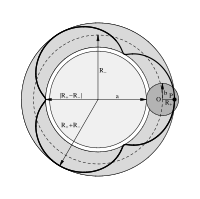
\includegraphics[width=0.5\linewidth]{Penning_trap_movement_general}
	\caption[Radial movement in Penning trap]{A general tragectory of an ion in a Penning trap, as seen from the direction of the $z$ axis. The parameters $R_-$ and $R_+$ are dependant on the initial conditions; $a$ and $b$ depend on  Figure taken from \cite{Charged_Particle_traps_Penning}.}
	\label{Fig:Penning_movement}
\end{figure}


As discussed in \cite{Charged_Particle_traps_Penning} and \cite{Penning_traps} several useful relations exist between the angular frequencies of the ion:

\begin{align}
	\omega_+ + \omega_- &= \omega_c
\label{Eq:Useful:cyclotron} \\
	2\omega_+\omega_- &= \omega_z^2
\label{Eq:Useful:cross}\\
	\omega_+^2 + \omega_-^2 + \omega_z^2 &= \omega_c^2
\label{Eq:Useful:squareSum}
\end{align}

It is useful to note that \eref{Eq:Useful:squareSum} holds even for slightly elliptic electrodes and misaligned magnetic field, called the invariance theorem\cite{Charged_Particle_traps_Penning,Single_ion_Penning}. Discussions for real world Penning traps and how to treat inhomogeneities in the magnetic, and imperfections in the electric field can be found in \cite{Charged_Particle_traps_Penning}, but these will not be included here.

\subsection{Paul trap}
\label{Trap:Paul}

The same geometry used in the Penning trap discussed in Section \ref{Trap:Penning} and shown in \figref{Fig:Penning} can be utilised with an oscillating electric field to create a trapping force. By applying a voltage of $U_0 + V_0\cos\left(\Omega t\right)$ a potential of the form

\begin{equation}
	\Psi = \frac{U_0 + V_0\cos\left(\Omega t\right)}{2 d^2}\left(2z^2 - x^2 - y^2\right)
	\label{Eq:PaulPot}
\end{equation}

can be created\footnote{Here $d$ has the same meaning it had in Section \ref{Trap:Penning}}\cite{Charged_Particle_traps_Paul,RF_Traps}. The resulting oscillations can be seen in \figref{Fig:PaulPot}. The relevant equations of motion for a particle with mass $M$ and charge $Q$ can be brought into the form:

\begin{figure}[t!]
	\centering
	\includegraphics[width=0.7\linewidth]{Paul_trap_pot}
	\caption[Paul trap potential oscillation]{Oscillation of the potential field within a Paul trap, where $T$ is the period of the oscillation. The time averaged force on a suitable particle will be pointing toward the trap's centre. Figure taken from \cite{Charged_Particle_traps_Paul}.}
	\label{Fig:PaulPot}
\end{figure}

\begin{equation}
	\der[2]{u_j}{t} + \left(a_j - 2q_j\cos\left(2\tau\right)\right) = 0
	\label{Eq:PaulEqMot}
\end{equation}

, where $j \in \left(x,y,z\right)$, $\tau = -\frac{1}{2}\Omega t$ and

\begin{figure}[t!]
	\centering
	\begin{subfigure}[b]{0.4\textwidth}
		\centering
		\includegraphics[width=\textwidth]{PaulStability1.pdf}
		\caption{Stability diagram for the Paul trap. Light grey areas represent axial, while dark grey areas mark radial stability.}
		\label{Fig:PaulStability:Wide}
	\end{subfigure}
	\hfill
	\begin{subfigure}[b]{0.5\textwidth}
		\centering
		\includegraphics[width=\textwidth]{PaulStability2.pdf}
		\caption{A closer view of the first stable region. Lines indicate constant values of $\beta_z$ and $\beta_r$; parameters in the solutions of \eref{Eq:PaulEqMot}\cite{Charged_Particle_traps_Paul}.}
		\label{Fig:PaulStability:First}
	\end{subfigure}
	\caption[Stability diagrams for a Paul trap]{Diagrams showing the stable combinations of parameters taken from \cite{Charged_Particle_traps_Paul}}
	\label{Fig:PaulStability}
\end{figure}

\begin{align*}
	a_x = a_y = - \frac{1}{2} a_z &= -\frac{4QU_0}{Md^2\Omega^2}\\
	q_x = q_y = - \frac{1}{2} q_z &= -\frac{2QV_0}{Md^2\Omega^2}
\end{align*}

As discussed in \cite{Charged_Particle_traps_Paul}, \cite{Single_trapped_ions} and \cite{RF_Traps}, solving \eref{Eq:PaulEqMot} leads to stability conditions for the trap pictured in \figref{Fig:PaulStability}. These can even be expanded so that - with careful choice of applied voltage - one can trap multiple species of ions\cite{Foot_two_freq_paul_trap}.

An other configuration in which radio-frequency traps are realised is the so called linear RF trap\cite{RF_Traps,Single_trapped_ions}. Such a configuration can be seen in \figref{Fig:LinearRF}. As noted in \cite{RF_Traps} and \cite{QI_Application} traps bearing similar geometry can be of particular interest in the field of quantum computation, as we will later see.


\begin{figure}[t!]
	\centering
	\includegraphics[width=0.5\linewidth]{linear_rf_trap}
	\caption[Linear RF trap diagram]{A schematic of a linear RF trap. Such a device is useful for constraining multiple ions in a single line. Illustration taken from \cite{Single_trapped_ions}.}
	\label{Fig:LinearRF}
\end{figure}


\section{Cooling techniques}
\label{Cooling}

To access the states of the ions, which are of interest to us we need to cool them drastically. While there are many ways of doing this, such as resistive cooling\cite{Cooling_techniques} we will be mainly focusing on resolved sideband cooling.

Before we can start resolved sideband cooling the ions, they would need to be prepared, generally using Doppler cooling. A more general outlook on it can be found in \cite{Foot} or \cite{Charged_Particle_traps_Cooling,Cooling_techniques} for ion traps, but has however an important idea has to be kept in mind for the case of the Penning trap. While the axial and cyclotron motions can be cooled by removing energy, the magnetron motion requires energy to be added, for the it to cool. It has been shown however that an intensity profile of $I(r) = I_0\left(1 + r/r_0\right)$ can be used to cool the magnetron and cyclotron modes can be cooled together\cite{Charged_Particle_traps_Cooling,Penning_Doppler_One_Laser}; a technique called axialisation may also be used in which an external field, oscillating with $\omega_c$ couples the magnetron and cyclotron motions together\cite{Penning_traps,Sideband_cooling_penning_trap}.

\subsection{Resolved sideband cooling}
\label{Cooling:Sideband}

While Doppler cooling can reach almost to absolute zero\cite{Foot}, many experiments require the system to be in the ground state of the motion\cite{Sideband_cooling_penning_trap,QIP_Trapped_ions}. To achieve such a state, resolved sideband cooling can be used\cite{Cooling_techniques,Ion_cooling}. An important  metric for the motion of the ion is the Lamb-Dicke parameter defined as: $\eta = k_L z_0$, where $k_L$ is the axial laser wavenumber and $z_0$ is the ground state spread\cite{Sideband_cooling_penning_trap}. For resolved sideband cooling $\eta < 1$, so that the ion's oscillation is contained within the laser's wavelength. An other important requirement is that the ion is in the strong binding regime, that is $\omega_0 > \gamma_n$, where $\omega_0$ is the transition frequency, and $\gamma_n$ is the spectral width of the oscillation\cite{Charged_Particle_traps_Cooling}.

A further improvement on this technique is if $\eta \ll 1$ for the system, which is called the Lamb-Dicke regime\cite{Charged_Particle_traps_Cooling}. In this state only the main transition and the immediate $\omega_0 \pm \omega_z$ sidebands are of interest. Considering an atom with two internal energy levels $A_0 = e$ and $A_1 = g$ and vibrational modes $n$, we can characterise the system by $\ket{A_i} \otimes \ket{n}$. By tuning a laser onto the first red sideband (i.e. $\omega_0 - \omega_z$), we can induce a transition $\ket{e,n} \rightarrow \ket{g,n-1}$, which will then relax with a high likelihood to $\ket{e,n-1}$\cite{Ion_cooling}.

As highlighted by \cite{Ion_cooling}, the requirement for a narrow transition makes it so that the ion will cool very slowly, as the lifetime of the state will be necessarily long. To combat this a higher lying state can be coupled, which has a transition to both the ground state and our metastable state, speeding up the process\cite{Charged_Particle_traps_Cooling,Ion_cooling}. While not discussed here an important experimental extension to sideband cooling is electromagnetically induced transparency (EIT)\cite{EIT_cooling,Ion_cooling,Charged_Particle_traps_Cooling}.

\section[QI Processing]{Quantum information processing with trapped ions}
\label{QI}

Trapped ions are of great interest from a quantum computational point of view\cite{QIP_Trapped_ions,QI_Application,Trapped_ion_qbit_toolbox,Cold_trapped_ions_QC}. The quantum information can be stored in various states, most importantly hyperfine and Zeeman states\cite{Trapped_ion_qbit_toolbox} or long lived, metastable optical states, such as the $3\text{d}^2\text{D}_{5/2}$ state of $^{40}\text{Ca}^+$ \cite{QIP_Trapped_ions,Trapped_Quantum_Computer}. This qubit state is then coupled with a short lived excited state using this short lived state as a readout transition, when the collapse of the qubit is desired\cite{Trapped_ion_qbit_toolbox}.

In a linear RF trap, multiple ions can be prepared, and since their motion is strongly coupled\cite{Trapped_ion_qbit_toolbox,QIP_Trapped_ions,QI_Application}, leading to an ideal situation, where the motional states, can be used to exchange quantum information between the ions in the system, allowing simple quantum gate operations such as the controlled NOT (CNOT) gate, in which the target qubit's state is rotated $180^\circ$ if the control qubit is in $\ket{\uparrow}$\cite{Trapped_ion_qbit_toolbox}. It can be shown that, while the Hilbert space in which the qubits reside is extensive ($2^N-1$) the system can be perfectly manipulated via a couple quantum operations, whose number is independent of the number of qubits\cite{Elementary_QGates}. 

An alternative to the Cirac-Zoller type gate interactions presented above, which couple $\sigma_z\otimes\sigma_z$, M\o{}lmer-S\o{}rensen gates, one of which is pictured in \figref{Fig:MolmerSorensen}\cite{Trapped_ion_qbit_toolbox} couple $\sigma_\phi\otimes\sigma_\phi$; these gates can used to create Bell states with $99\%$ fidelity.

\begin{figure}[t!]
	\centering
	\includegraphics[width=0.7\linewidth]{Molmer-Sorensen}
	\caption[M\o{}lmer-S\o{}rensen gate]{M\o{}lmer-S\o{}rensen gate operation. A bichromatic laser is used to probe near both the blue and red sidebands, coupling $\ket{\downarrow\downarrow}$ and $\ket{\uparrow\uparrow}$ qubit states. Illustration taken from \cite{Trapped_ion_qbit_toolbox}}
	\label{Fig:MolmerSorensen}
\end{figure}

The biggest issue in quantum computing is decoherence; this phenomenon couples the state of the qubits to the environment destroying the quantum state and ruining the result\cite{QI_Application}. The fidelity of such gate operations however increased significantly during the last few years, being around $90\%$ in 2013\cite{Trapped_ion_qbit_toolbox} and by 2021 raising to excess of $99\%$\cite{Trapped_Quantum_Computer}; this decoherence is mostly from the heating of the ions in their motional states\cite{Trapped_Quantum_Computer}.

\section{Conclusion}
\label{Conclusion}

The main focus points of the project will have to primarily be the accurate modelling of the heating effects of the trap, given that it is the biggest limit on coherence in similar experiments\cite{Trapped_Quantum_Computer}. A secondary consideration, which was only mentioned, because of its length is the imperfections in the trapping potential\cite{Charged_Particle_traps_Penning,Charged_Particle_traps_Paul}. Finally the inter ionic interactions, should be modelled precisely, as that interaction shares the information between atoms in many quantum gates, that are of interest\cite{Trapped_ion_qbit_toolbox}.
 

%% bibliography
\bibliographystyle{ieeetr}
\bibliography{sources}

\end{document}